%%%%%%%%%%%%%%%%%%%%%%%%%% author.tex %%%%%%%%%%%%%%%%%%%%%%%%%
%
% sample root file for your contribution to a "contributed book"
%
% "contributed book"
%
% Use this file as a template for your own input.
%
%%%%%%%%%%%%%%%%%%%%%%%% Springer-Verlag %%%%%%%%%%%%%%%%%%%%%%%%%%

\documentclass{svmult}

\usepackage{amsmath}
\usepackage{amsfonts}
%\usepackage{amssymb}
\usepackage{color}
\usepackage{url}
\usepackage{verbatim}
\usepackage[dvipdfm]{graphicx} % add

%\usepackage{makeidx}         % allows index generation
\usepackage{graphicx}        % standard LaTeX graphics tool
                             % when including figure files
%\makeindex             % used for the subject index
                       % please use the style sprmidx.sty with
                       % your makeindex program

%%%%%%%%%%%%%%%%%%%%%%%%%%%%%%%%%%%%%%%%%%%%%%%%%%%%%%%%%%%%%%%%%%%%%
%\newtheorem{theorem}{Theorem}[section]
%\newtheorem{conjecture}[theorem]{Conjecture}
%\newtheorem{corollary}[theorem]{Corollary}
%\newtheorem{proposition}[theorem]{Proposition}
%\newtheorem{lemma}[theorem]{Lemma}
%\newdef{definition}[theorem]{Definition}
%\newdef{remark}[theorem]{Remark}

% \def\F2{{\mathbb F}_2}
% \def\wt{{\rm wt}}
% \def\wo{{\rm wt}_o}
% \def\wf{{\rm wt}_f}
% \def\UL{{\rm ul}}
% \def\bx{{{\mathbf x}}}
% \def\by{{{\mathbf y}}}
% \def\bz{{{\mathbf z}}}
% \def\bw{{{\mathbf w}}}
% \def\bu{{{\mathbf u}}}
% \def\im{{\mathrm{Im}}}
% \def\ker{{\mathrm{Ker}}}
% \def\id{{\mathrm{Id}}}
% \def\tr{{\mathrm{tr}}}

\def\bbf2{\ifmmode\mathbb{F}_2\else$\mathbb{F}_2$\fi}%
%\newcommand{\bbf2}{{\ifmmode \mathbb{F}_2 \else $\mathbb{F}_2$ \fi}}

%%%%%%%%%%%%%%%%%%%%%%%%%%%%%%%%%%%%%%%%%%%%%%%%%%%%%%%%%%%%%%%%%%%%%
\begin{document}
%\newcommand{\bbf2}{\ifmmode \mathbb{F}_2 \else $\mathbb{F}_2$ \fi}
\newcommand{\mmod}{\textrm{mod}\,}
%%%%%%%%%%%%%%%%%%%%%%%%%%%%%%%%%%%%%%%%%%%%%%%%%%%%%%%%%%%%%%%%%%%%%

%\title*{Ultra-Fast Low-Discrepancy Points}
%\titlerunning{Fast Points}
%\title*{A uniform real random number generator obeying the IEEE 754
%  format using an affine transition}
\title*{A PRNG specialized in double precision floating point numbers
  using an affine transition}

\titlerunning{A PRNG specialized in double precision floating point numbers}

% \author{
% Usain Bolt\inst{1}\and
% Michael Phelps\inst{2}
% }
%\author{Mutsuo Saito\inst{1}\and
%Makoto Matsumoto\inst{2}}

\author{Mutsuo Saito \and Makoto Matsumoto}

% Use \authorrunning{Short Title} for an abbreviated version...
%
% \institute{
% Departement of Superhumans \\
% Lightning Yellow High School\\
% Kingston, Jamaica\\
% \url{http://en.wikipedia.org/wiki/Usain_Bolt}
% \and
% Deep Blue Swimming Pool \\
% University of Baltimore, USA \\
% \url{http://en.wikipedia.org/wiki/Michael_Phelps}
% }
\institute{
Mutsuo Saito \at Department of Mathematics,
Graduate School of Science, Hiroshima University, Hiroshima, Japan, 
\email{saito@math.sci.hiroshima-u.ac.jp} \\
\and 
Makoto Matsumoto \at 
Department of Mathematics, 
Graduate School of Science, Hiroshima University, Hiroshima, Japan,
\email{m-mat@math.sci.hiroshima-u.ac.jp} \\
}

\maketitle
%%%%%%%%%%%%%%%%%%%%%%%%%%%%%%%%%%%%%%%%%%%%%%%%%%%%%%%%%%%%%%%%%%%%%
            
\abstract{
  We propose a pseudorandom number generator specialized to
  generate double precision floating point numbers,
  which generates pseudorandom 52-bit patterns supplemented
  by a constant most significant 12-bit (sign and exponent), so 
  that the concatenated 64-bit represents a floating
  point number obeying the IEEE 754 format. To keep the constant
  part, we adopt an affine transition function instead of 
  usual $\mathbb{F}_2$-linear transition, and extend algorithms
  computing the period and the dimensions of equi-distribution
  to the affine case.
  The resulted generator generates double precision
  floating point numbers faster 
  than Mersenne Twister generates those of 32-bit precision.
}
%%%%%%%%%%%%%%%%%%%%%%%%%%%%%%%%%%%%%%%%%%%%%%%%%%%%%%%%%%%%%%%%%%%%%

\section {Introduction}
\label{sec:intro}

In \cite{SFMT}, we proposed a fast version of the Mersenne twister (MT) of \cite{MT},
that exploits the single instruction multiple data \cite{wiki:SIMD} (SIMD) feature of some
recent CPUs, which processes 128-bit at a time. 
This new pseudorandom number generator (PRNG), named SFMT (which stands for SIMD-oriented
fast Mersenne twister), is faster than the original MT and also has better
equidistribution. The proposal of \cite{SFMT} also features a block generation
procedure, which returns a large array of pseudorandom numbers at
each call.

%We are interested in scientific simulations, and most scientific
%Monte-Carlo simulation requires great deal of floating point
%pseudorandom numbers. 

In this article, we propose PRNGs
specialized in generating floating point numbers, which 
we call dSFMT (double precision floating point SFMT).
It generates a sequence of 64-bit patterns with constant 
12 most significant bits (MSBs), so that each of 64-bit patterns
represents a double precision floating point numbers in a fixed 
interval in the standard IEEE754 format.
Instead of usual ${\mathbb F}_2$-linear transition function, 
we adopt ${\mathbb F}_2$-affine transition function to keep the
fixed constant in the 64-bit (\S\ref{sec:affine}). We extended
some of the existing algorithms to compute the period and distribution 
to the affine case. 
As a result, we implemented this type of generators whose periods 
are multiples of 
6 Mersenne primes from $2^{521}-1$ to $2^{19937}-1$, respectively.
These generators are shown to be faster than MT, SFMT and WELL generators,
and have satisfactorily high dimensions of equidistribution 
(much higher than MT, but lower than WELL which attains the theoretical bounds).


%%%%%%%%%%%%%%%%%%%%%%%%%%%%%%%%%%%%%%%%%%%%%%%%%%%%%%%%%%%%%%%%%%%%%
\section{Generating floating point numbers}
\label{sec:floating}\label{sec:ieee}

Usually, floating point pseudorandom numbers are obtained by
converting integer pseudorandom numbers. 
One may consider recursion in floating
point numbers for PRNG, but it may accumulate approximation errors.
Since the rounding-off is not standardized, the generated
sequence often depends on CPUs. 
Consequently, usual PRNGs generate integer random numbers by integer recursion,
and converts them 
to floating point numbers by multiplying a constant.
However, this method requires a conversion from an integer to
a floating point number, which consumes about 50\% of the cpu-time
in the generation, according to our experiments using
the 64-bit MT \cite{MT64}.

A faster conversion is given by bit operations
fitting to a standard floating point format. We recall
the most widely-used standard, 
IEEE Standard for Binary Floating-Point Arithmetic (ANSI/IEEE Std
754-2008) \cite{ieee754}, which we shall refer as IEEE 754.
The standard was defined in 1985 and revised
in 2008, and we here treat the 64-bit binary format valid 
for both.
The 64-bit are separated in to 
the sign bit (the most significant bit, MSB),
the exponent 11 bit (the next significant 11 bits representing
an integer between $0$ to $2047$, denoted by $e$)
and the rest 52 fraction bits (representing a real number in $[1,2)$: 
52-bit pattern \texttt{xxx}$\ldots$ is interpreted
as a binary floating number 1.\texttt{xxx}$\ldots$, 
denoted by $f$).
When $0<e<2047$, the 64-bit
represents a floating point number
$\pm f \times 2^{e - 1023}$ with the sign determined by the
sign bit.
Thus, if the sign bit is 0 and $e=1023$ (or equivalently 
the 12 MSBs being \texttt{0x3ff} in hexadecimal form),
then the represented number is in $[1,2)$. If the 52-bit fraction part 
is uniformly randomly chosen, 
then the represented number is uniformly randomly distributed over $[1,2)$
with 52-bit precision.
In C-language, this conversion of a 64-bit integer \texttt{x} is described as follows:
\begin{verbatim}
   x = (x >> 12) | 0x3FF0000000000000ULL;
   y = *((double *)&x);
\end{verbatim}
where the first line shifts \texttt{x} to the right by 12 bits
and set the 12 MSBs to the constant \texttt{0x3ff}, 
and the second line regards the 64-bit pattern as an IEEE 754 format.
This method is less portable than the conversion by multiplication,
depending on a particular format,
but consumes only 5\% to 10\% of the cpu-time for the conversion,
according to our experiments with the 64-bit MT.
This method goes back to at least 1997: Agner Fog used this method in
his open source library \cite{web:Fog}, and others seemed to invent
it independently, too.

A pseudorandom number $r$ in $[1,2)$ can be converted into 
$[0,1)$ (respectively $(0,1]$) by taking $r-1$ (respectively $1-r$).
In practice, it is often the case that 
random numbers $r$ in the range $[1,2)$ can be used
without converting into $[0,1)$:
for example, the Box-Muller transformation 
converts two uniform random numbers $s_1,s_2$ in $[0,1)$ 
into two normally distributed numbers
$$
\sqrt{-2 \log(1-s_1)}\sin (2 \pi s_2), 
\sqrt{-2 \log(1-s_1)}\cos (2 \pi s_2).
$$
If $r_1, r_2$ are two uniform random numbers in $[1,2)$,
then the conversion can be done by 
$$
\sqrt{-2 \log(2-r_1)}\sin (2 \pi r_2), 
\sqrt{-2 \log(2-r_1)}\cos (2 \pi r_2).
$$ 

%%%%%%%%%%%%%%%%%%%%
\section{LFSR with lung}
\label{sec:pulmonary}
Our proposal is to use a linear recursion over ${\mathbb F}_2$
to generate a sequence of 64-bit patterns with
12 MSBs being \texttt{0x3ff} as above,
by a Linear Feedback Shift Register (LFSR)
with additional memory called `lung.'
We identify the set of bits \{0, 1\} with the two element field ${\mathbb F}_2$.
This means that every arithmetic operation is done modulo 2.  
A $b$-bit register or memory is identified with a horizontal
vector in ${\mathbb F}_2^b$, and $+$ denotes the sum as vectors (i.e.,
bit-wise exclusive or). We consider an array of $b$-bit integers of
size $N$ in
computer memory as the vector space $({\mathbb F}_2^{b})^N$.

An LFSR method is to generate a sequence $\mathbf{w_0}$,$\mathbf{w_1}$,
$\mathbf{w_2},...$ of elements ${\mathbb F}_2^b$ by a recursion
\[ \mathbf{w}_{i+N} = g(\mathbf{w}_{i}, ..., \mathbf{w}_{i + N-1}), 
\quad (i=0,1,2,\ldots)
\]
where $g$ is an ${\mathbb F}_2$-linear map $({\mathbb F}_2^{b})^N \rightarrow
{\mathbb F}_2^b$.  In the implementation, this recursion is computed by using
an array \texttt{W[0..N-1]} of $N$ words of $b$-bit size, by the
simultaneous substitutions

\begin{multline*}
    \texttt{W[0]} \leftarrow \texttt{W[1]},\ 
    \texttt{W[1]} \leftarrow \texttt{W[2]}, \ldots,
    \texttt{W[N-2]} \leftarrow \texttt{W[N-1]}, \\  
    \texttt{W[N-1]} \leftarrow
    g(\texttt{W[0]},\ldots,\texttt{W[N-1]}). 
  \end{multline*}

The first $N-1$ substitutions shift the content of the array, hence
the name of LFSR.  Note that in the implementation we may use an
indexing technique to avoid computing these substitutions, see
\cite[P.28 Algorithm A]{knuth:bible}.  Before starting the generation,
we need to set some values to the state array, which is called the
initialization. Mersenne Twister \cite{MT} (MT) is such an example.

An LFSR with lung is to generate a sequence
$\mathbf{w_0}$,$\mathbf{w_1}$, $\mathbf{w_2},...$ of elements
${\mathbb F}_2^b$ by a recursion
\begin{eqnarray}
  \mathbf{w}_i &=& g(\mathbf{w}_{i-N+1}, ..., \mathbf{w}_{i-1},
  \mathbf{u}_{i-1}), \label{eq:recursion} \\
  \mathbf{u}_i &=& h(\mathbf{w}_{i-N+1}, ..., \mathbf{w}_{i-1},
  \mathbf{u}_{i-1}). \label{eq:lung}
\end{eqnarray}
where $g$ and $h$ are ${\mathbb F}_2$-linear maps $({\mathbb F}_2^{b})^N \rightarrow
{\mathbb F}_2^b$ and $\mathbf{w}_i, \mathbf{u}_i \in {\mathbb F}_2^b$.  In the
implementation, $\mathbf{w}_i$'s are kept in an array
\texttt{W[0..N-1]}, and $\mathbf{u}_i$
is (expected to be) kept in a register of
CPU, which is called the {\em lung}. We denote the register
by \texttt{U}. The first line (\ref{eq:recursion})
renews the array \texttt{W[0..N-1]}, and the second line (\ref{eq:lung}) renews
the register (lung) \texttt{U}.
The idea of LFSR with lung appeared in the talk of Hiroshi
Haramoto in a conference MCM 2005, and used in WELL PRNG \cite{WELL} in 2006.
The lung realizes a short feedback loop, which improves
some measures of randomness such as higher dimensional 
equidistributions and the density of nonzero coefficients
in the characteristic polynomial.

\section{Affinity introduced by the constant part}\label{sec:affine}
Our idea is to design the functions $g$ and $h$ in 
the recursion (\ref{eq:recursion})
(\ref{eq:lung}) for LFSR with lung, so that if the initial 
values $\mathbf{w}_0, \ldots, \mathbf{w}_{N-1}$ are set to 
have \texttt{0x3ff} at their 12 MSBs, then the following 
$\mathbf{w}_i$ have the same property, regardlessly of 
the value of $\mathbf{u}_0$. According to our experiments, 
this method is 5\% to 10\% faster than the bit-masking
conversion explained in \S\ref{sec:floating}. 

A new difficulty in this approach is that 
the state transition is far from being maximal periodic.
A linear state transition function is said to be
maximal periodic, if every non-zero state lies on
the same orbit. The existence of the constant implies that, if 
the initial state is chosen as above, then 12 MSBs 
of each member of the array of \texttt{W[0..N-1]}
are constant in the orbit, and the transition can not be
maximal periodic. This makes it difficult to apply
standard techniques to compute the period and
high-dimensional equidistribution property.

A natural solution to this problem is to redefine
the state space by excluding the constant part, 
and consider the transition function as an 
affine function.
More concretely, let $\mathbf{w}_{i}'$ denote the
lower 52-bit of $\mathbf{w}_i$. Since the upper 12-bit
is a constant, the recursion
formula (\ref{eq:recursion}), (\ref{eq:lung})
can be described by
\begin{eqnarray}
  \mathbf{w}_i' &=& g'(\mathbf{w}_{i-N+1}', ..., \mathbf{w}_{i-1}',
  \mathbf{u}_{i-1}), \label{eq:recursion-dash} \\
  \mathbf{u}_i &=& h'(\mathbf{w}_{i-N+1}', ..., \mathbf{w}_{i-1}',
  \mathbf{u}_{i-1}). \label{eq:lung-dash}
\end{eqnarray}
Here, it is easy to see that the linearity of $g$ (resp.\ $h$)
implies the affinity of $g'$ (resp.\ $h'$). (Here affine means
linear plus a constant.)

Let $b_w$ denote the number of variable bits 
in each \texttt{W[i]} (52 in the above case), 
and $b_u$ denote the number of bits in the 
lung \texttt{U}.
This LFSR with lung (not linear but affine)
is considered as an automaton, with the state space 
$S={\mathbb F}_2^{b_u + b_w \times (N-1)}$.
The state transition function $F: S \to S$ is given by
\begin{equation*}
  \begin{split}
    (\mathbf{w}_0', &\ldots,\mathbf{w}_{N-2}', \mathbf{u}_0) \\
    &\mapsto 
    (\mathbf{w}_1',\ldots,\mathbf{w}_{N-2}',
    g'(\mathbf{w}_0',\ldots,\mathbf{w}_{N-2}', \mathbf{u}_0),
    h'(\mathbf{w}_0',\ldots,\mathbf{w}_{N-2}', \mathbf{u}_0)).
  \end{split}
\end{equation*}
As a $b_w$-bit vector generator (i.e., removing
the constant bits), the output function is 
\[
  o: S \to {{\mathbb F}_2}^{b_w}; \quad
  (\mathbf{w}_0', \ldots, \mathbf{w}_{N-2}', \mathbf{u}_0) 
  \mapsto \mathbf{w}_0'.
\]

%We shall consider the variable bits in the array and the lung
%as the state space of the PRNG.
Now, both $F$ and $o$ are not linear
but affine. Namely, they have the form 
$x \mapsto Ax+c$ where $x$ is a vector, $A$ is an
$\mathbb{F}_2$ matrix, and $c$ is a constant vector.
(If $c=0$, it is linear.)

%%%%%%%%%%%%%%%%%%%%
\section{Reduction from affine to linear: fixed points}
\label{sec:fixed-point}
Let $f$ denote the linear part of $F$,
namely, put $c:=F(0)$ and 
\begin{equation}
F(x) = f(x) + c
\end{equation}
with linear $f: S \to S$. 
If $F$ has a fixed point
$F(z)=z$, then $F(x-z)=f(x-z)+c=f(x)-z$, and
consequently $F^n(x-z)=f^n(x)-z$.
Thus, for the state transition $x_0,x_1,x_2,\ldots$ by $F$,
its translation $x_0+z, x_1+z, \ldots$ by the constant $z$
is obtained by the linear state transition $f$, hence can be analyzed
by the existing methods. 
Since the period and the distribution property of the
sequence is unchanged by a parallel translation, 
computation of those for the affine $F$ is 
reduced to those for the linear $f$. If $f$ has the maximal period,
then the equidistribution property can be computed as usual.

The equation $F(z)=z$ is equivalent to $(f-\textrm{Id})(z)=c$,
where $\textrm{Id}$ denotes the identity transformation on 
$S$.
Thus, a fixed point exists 
if the characteristic polynomial $\chi_f$ of $f$ 
does not have 1 as a root, 
in particular if irreducible with degree $\geq 2$.

\section{Reducible transition function in affine case}
\label{sec:RTM}
Usually, to assure the period, we need to check 
the primitivity of $\chi_f$.
This is often computationally difficult, 
since we need the integer factorization of
$2^{\deg(\chi(t))}-1$, which is hard if the degree is high (say, $>10000$).
There are two methods to avoid this: (1) to tune the size of the state space
to be a Mersenne exponent (i.e. a prime number $p$
such that $2^p-1$ is also prime) where $2^{\deg(\chi(t))}-1$ is a prime,
and (2) to use $f$ such that $\chi_f$ has an irreducible factor
of a Mersenne prime degree denoted by $p$. We here adopt the latter
method, named reducible transition method (RTM) in \cite{SFMT}. 
This is advantageous over
the former in the generation speed, because of no need of discarding
a part of the state array (as was required in MT \cite{MT} and WELL \cite{WELL}).
Note that this idea appeared in somewhat different purposes previously in 
 \cite{FUSHIMI90}\cite{BRENT}\cite{BRENT-PRIM}.
 
We here recall RTM very briefly. 
Let $f:S \to S$ be an ${\mathbb F}_2$-linear transition function,
$o:S \to O$ be an ${\mathbb F}_2$-linear output function.
Assume that
a linear transition function $f:S \to S$ has a decomposition
$S=V_p \oplus V_r$, $f=f_p \oplus f_r$ with $f_p:V_p \to V_p$,
$f_r:V_r \to V_r$. In other words, $f$ is the 
combined generator obtained from the two generators 
$(f_p, V_p, o_p)$ and $(f_r, V_r, o_r)$,
in the sense of \S2.3 of \cite{F2RNG-LEcuyer}. A linear output function
$o:S \to O$ is then the sum of there restrictions $o_p:V_p \to O$ and
$o_r:V_r \to O$. The output of the combined generator is obtained by
taking xor of the outputs of each generator.
The period of the combined generator $(f,S,o)$ is the least common multiple 
of the two generators. Thus, once we know that $(f_p,V_p,o_p)$ has a large 
period, then the combined generator has at least that period.

Our strategy is to fix a Mersenne prime $p$, to determine the
size $N$ of the state array so that $p \leq \dim S$, and then
search for parameters with a factorization 
$\chi_f=\phi_p \phi_r$, where $\phi_p$ is irreducible of degree $p$
and $\phi_r$ has degree $r$ with $r<p$. Then, it is automatic to have
a decomposition $S = V_p \oplus V_r$ into $p$-dimensional and 
$r$-dimensional subspaces, so that the restriction
$f_p$ (respectively $f_r$) of $f$ to $V_p$ (respectively to $V_r$)
has the characteristic polynomial $\phi_p$ (respectively $\phi_r$).
Once we have such decomposition, then the component $f_p:V_p \to V_p$ 
has the Mersenne exponent dimension $p$, 
and hence an existing method searches for the parameters that assure 
the period of $2^p-1$. Then we can assure $2^p-1$ as the lower bound of the
period of the combined generator, provided that the initial state 
$s = s_p \oplus s_r \in S = V_p \oplus V_r$ has non zero component 
$s_p \neq 0$.

In the case of affine transition $F(x)=f(x)+c$, we assume 
that its linear part $f$ satisfies the above factorizing condition
$\chi_f=\phi_p\phi_r$. 
Let us decompose $c=c_p\oplus c_r$ and $x=x_p\oplus x_r$
along $V_p\oplus V_r$, then
\begin{equation}\label{eq:decomp-F}
F(x)=f(x)+c=(f_p(x_p)+c_p) \oplus (f_r(x_r)+c_r)=:F_p(x_p)\oplus F_r(x_r).
\end{equation}
This implies that the affine generator $(F, S, o)$ is 
obtained by combining two affine generators 
$(F_p, V_p, o_p)$ and $(F_r, V_r, o_r)$. 
Now $f_p$ is irreducible, and the fixed point argument in 
\S\ref{sec:fixed-point} reduce the computation of the periods
and the high-dimensional equidistribution property for $F_p$
to those for $f_p$.
%Note that the dimensions of the equidistribution of the combined generator
%is bounded from below by those of the component generators 
%\cite[Proposition 1]{LEcuyer-combdif}\cite{SFMT}, and hence
%those for $(f_p,V_p,o_r)$ give lower bounds on those for
%the desired generator $(F, S, o)$. This will be treated later.

\section{Period certification}
\label{sec:PCV}
We explain how to choose parameters 
realizing the period $2^p-1$, for a given
Mersenne exponent $p$.
For the linear transition function, the method is 
described in \cite{SFMT}, which we briefly 
recall.
Let 
$N$ be the smallest length of the array such that
the dimension of the state space 
$S={\mathbb F}_2^{b_u + b_w \times (N-1)}$
is greater than or equal to $p$. Thus, 
$r:=\dim S - p < b_w$ holds.

We randomly choose parameters for the recursion 
(\ref{eq:recursion-dash}) and
(\ref{eq:lung-dash}). Let $F:S \to S$ be the 
corresponding affine transition function, and $f:S \to S$ be
its linear part. We compute the characteristic
polynomial $\chi_f(t)$ by using Berlekamp-Massey algorithm, and
check whether it decomposes to 
\[
\chi_f=\phi_p \phi_r
\]
where $\phi_p$ is a primitive polynomial of degree $p$
and $\phi_r$ is a polynomial of degree %$r = wN-p$.
$r:=\dim S -p < b_w$. We assume $r<p$, which is natural
in our context where $p$ is large, and also $b_w\leq b_u$,
since $b_w$ is the number of the non-constant part in 
a $b_u$-bit word.
We continue the random search of parameters, 
until we obtain a primitive $\phi_p$.

Once we found such a set of parameter, then we have
$S=V_p \oplus V_r$ and the projector $P_p: S \to V_p$.
To assure the period of a multiple of $2^p-1$ for the initial state $s \in S$,
it suffices to assure $s_p:=P_p (s) \neq 0$. 
In the implementation, to compute $P_p(s)$ is a time-consuming
procedure in the initialization. Instead, we propose the 
following method, named Period Certification Vector (PCV) method,
by which the period is certified by looking at one word in the state.

Let $V_U$ denote the $b_u$-dimensional vector space corresponding to the lung 
\texttt{U} in (\ref{eq:lung-dash}). To certify the period for
the initial state $s \in S$, it suffices to show that
$s \notin V_r$. Let $\pi:S \to V_U$ be the projection obtained
by extracting the lung from the state space $S$. Since we assumed
$b_u=\dim (V_U)>r$, the image $\pi (V_r)$ is a proper subspace of $V_U$.
Hence, there is a nonzero vector $q$ in $V_U$ which is orthogonal
to every vector in $\pi (V_r)$. We call such a vector {\em the period certification vector} (PCV).
For a given initial state $s$, if the inner product $\pi(s)\cdot q$ is nonzero,
then $\pi(s) \notin \pi(V_r)$ and hence $s \notin V_r$, and the period is certified. If
the inner product is zero, then we make the inner product nonzero by reversing 
appropriate one bit in $\pi(s)$.

The period certification for affine case easily reduces to the linear case. 
Let $z_p \in V_p$ be a fixed point of $F_p$. For the initial state $s \in S$,
it suffices to show that $s-z_p \notin V_r$ to assure the period. This 
can be done by precomputing $\pi(z_p)$, and check that 
$(\pi(s)-\pi(z_p))\cdot q \neq 0$. In this method, only two
constant $b_u$-bit words $\pi(z_p)$ and $q$ need to be precomputed
and stored, and at the initialization stage, only the last inner-product
is necessary to compute.

%%%%%%%%%%%%%%%%%%%%%%%%%%%%%%%%%%%%%%%%%%%%%%%%%%%%%%%%%%%%%%%%%%%%%
\section{Computation of the dimension of equidistribution}
\label{sec:DE}
We briefly recall the definition of dimension of 
equidistribution (cf. \cite{CLT}\cite{COMBTAUS}\cite{SFMT}).
%The version used here and its background are described in \cite{SFMT}. 
\begin{definition}\label{def:DE}
Let $F:S \to S$ be an affine transition function over $\mathbb{F}_2$.
Let $v$ be an integer, and $o:S \to {\mathbb F}_2^v$ be a $v$-bit
affine output function. The generator $(S, F, o)$ is said to be 
$k$-dimensionally equidistributed, if the map
$$
 S \to ({\mathbb F}_2^v)^k, \quad s \mapsto (o(s),o(F(s)), o(F^2(s)),\ldots,o(F^{k-1}(s)))
$$
is surjective.
The largest value of such $k$ is called the dimension 
of equidistribution (DE).
\end{definition}
For a $b$-bit integer generator, its {\em dimension of 
equidistribution at $v$-bit accuracy} $k(v)$
is defined as the DE of the $v$-bit sequence, obtained by extracting
the $v$ MSBs from each of the $b$-bit integers.

Let $P=2^p-1$ be the period of the generated sequence.
Then, there is an upper bound
$k(v) \leq \lfloor p / v \rfloor$,
and their gap $d(v)$ is 
called the dimension defect at $v$ of the sequence,
and their sum $\Delta$ over $v=1,\ldots,b$ is called
the total dimension defect, namely: 
\begin{equation}\label{eq:total-dim-difect}
d(v):=\lfloor p / v \rfloor -k(v) 
\mbox{ and } \Delta:=\sum_{v=1}^b d(v).
\end{equation}
%The summation of all the dimension defects at
%$1 \leq v \leq w$ is called the total dimension defect, 
%denoted by $\Delta$.
% We may compute $k(v)$ by standard linear algebra.
% We used a more efficient algorithm based on 
% a weighted norm,
% %{\em weighted lattice method} to compute $k'(v)$,
% generalizing \cite{CLT}. This will be written 
% somewhere else,
% because of lack of space. HARASE
We adopt RTM as in \S\ref{sec:RTM}, and 
the dimensions of the equidistribution of 
the larger component $(F_p, V_p, o_p)$ gives the 
lower bound of these dimensions \cite{LEcuyer-combdif}
\cite{SFMT}. Accordingly, we define $k(v)$ and $d(v)$ of
RTM to be those for this larger component. Let $f_p$
be the linear part of $F_p$.
Since $\chi_{f_p}$ is irreducible, there is a fixed point
of $F_p$ as explained in \S\ref{sec:fixed-point}. Thus,
computation of $k(v)$ for $F_p$ is reduced to 
that for the linear part $f_p$, which was done in \cite{SFMT}.

%There is a difficulty in computing $k(v)$ when 
%a 128-bit vector generator is used as a 32-bit 
%(or 64-bit) vector generator. This is solved by
%using weighted norm (see \cite{SFMT}\cite{thesis:saito}).

% SFMT generates a sequence
% $\mathbf{x}_0, \mathbf{x}_1, \mathbf{x}_2, \ldots$ of 128-bit integers. 
% Then, they are converted to a sequence of 32-bit integers
% $\mathbf{x}_0[0], \mathbf{x}_0[1], \mathbf{x}_0[2], \mathbf{x}_0[3], \mathbf{x}_1[0], \mathbf{x}_1[1],\ldots$,
% where 
% $\mathbf{x}[0]$ is the 32 LSBs of $\mathbf{x}$, 
% $\mathbf{x}[1]$ is the 33rd--64th bits,
% $\mathbf{x}[2]$ is the 65rd--96th bits,
% and $\mathbf{x}[3]$ is the 32 MSBs. 
% %(This is called the 
% %little-endian system, see 
% %\cite{wiki:endian}).
% %for the notion of endianness, 
% %and \S\ref{sec:portability} for
% %an implementation in a big-endian system). 

% Then, we need to modify the model automaton
% as follows.
% The state space is $S':=S \times \{0,1,2,3\}$,
% the state transition function $f':S' \to S'$ is
% $$
% f'(s,i):=
% \left\{
% \begin{array}{cl}
% (s, i+1) & (\mbox{ if $i<3$}), \\
% (f(s), 0) & (\mbox{ if $i=3$}) \\
% \end{array}
% \right.
% $$
% and the output function is 
% $$o': S' \to {\mathbb F}_2^{32},\  ((\mathbf{w}_0,\ldots,\mathbf{w}_{N-1}),i) \mapsto \mathbf{w}_0[i].$$

% We fix $1\leq v \leq w$, and let $o_k(s,i)$ be the $k$-tuple
% of the $v$ MSBs of the consecutive $k$-outputs from 
% the state $(s,i)$.
% \begin{proposition}
% Assume that $f$ is bijective.
% Let $k'=k'(v)$ denote the maximum $k$ 
% such that 
% \begin{equation}\label{eq:chi-k-i}
% %o_k(-,i): V_p \subset S \to {\mathbb F}_2^{kv}, \quad s \mapsto o_k(s,i)
% o_k(-,i): V_p \to {\mathbb F}_2^{kv}, \quad s \mapsto o_k(s,i)
% \end{equation}
% are surjective for all $i=0,1,2,3$. 
% %Take the initial state $s$ satisfying $s_p \neq 0$.
% Take an initial state $s$ satisfying $s_p \neq 0$.
% Then, the 32-bit output sequence is at least $k'(v)$-dimensionally
% equidistributed with $v$-bit accuracy with defect ratio
% $2^{-p}$.

% Moreover, if $4 < k'(v)+1$, then  
% for any initial state with $s=s_p \neq 0$
% (hence $s_r=0$), the dimension of equidistribution
% with defect ratio $2^{-p}$ is exactly $k'(v)$.
% \end{proposition}
% \begin{proof}
% Take $s \in S$ with $s_p \neq 0$. Then, the 
% orbit of $s$ by $f$ has the form of
% $(V_p - \{0\}) \times U \subset V_p \times V_r$,
% since $p>r$ and $2^p-1$ is a prime.
% %Since the first component of the product has
% %odd order, the orbit of $f'$ has the form of
% %$(V_p - \{0\}) \times U' \times \{0,1,2,3\} \in S$.
% The surjectivity of the linear mapping $o_{k'}(-,i)$
% implies that the image of 
% $$
% o_{k'}(-,i): V_p \times U \to {\mathbb F}_2^{kv}
% $$
% is $m\cdot {\mathbb F}_2^{kv}$ as a multi-set for some $m$.
% The defect comes from $0 \in V_p$, whose ratio
% in $V_p$ is $2^{-p}$. Then the first statement follows,
% since $W_{k'}(\chi)$ is the union of the images
% $o_{k'}(-,i)((V_p-\{0\})\times U)$ for $i=0,1,2,3$.

% For the latter half, we define
% $L_i$ as the multiset of the image of 
% $o_{k'+1}(-,i): V_p \to {\mathbb F}_2^{(k'+1)v}$.
% Because of $s_r=0$, we have $U=\{0\}$, and
% the union of $(L_i-\{0\})$ $(i=0,1,2,3)$ as a multi-set is 
% $W_{k'+1}(\chi)$. If the sequence is $(k'+1)$-dimensionally
% equidistributed, then the multiplicity of
% each element in $W_{k'+1}(\chi)$ is at most
% $2^p\times 4/ 2^{(k'+1)v}$.

% On the other hand, the multiplicity of 
% an element in $L_i$ is equal to 
% the cardinality of the kernel of $o_{k'+1}(-,i)$.
% Let $d_i$ be its dimension. Then by the dimension theorem,
% we have $d_i \geq p-(k'+1)v$, and the equality
% holds if and only if $o_{k'+1}(-,i)$ is 
% surjective.
% Thus, if there is a nonzero element 
% $x \in \cap_{i=0}^3{L_i}$, then its multiplicity
% in $W_{k'+1}(\chi)$ is no less than 
% $4 \times 2^{p-(k'+1)v}$, and since
% one of $o_{k'+1}(-,i)$ is not surjective
% by the definition of $k'$, its multiplicity
% actually exceeds $4 \times 2^{p-(k'+1)v}$,
% which implies that the sequence is not
% $(k'+1)$-dimensionally equidistributed, and
% the proposition follows. Since the codimension 
% of $L_i$ is at most $v$, 
% that of $\cap_{i=0}^3{L_i}$ is at most $4v$.
% The assumed inequality on $k'$ implies the existence
% of nonzero element in the intersection.
% %
% %Since the codimension of 
% %each $L_i$ is at most $v$, the codimension of
% %$\cap_{i=0}^3{L_i}$ is at most $4v$. The inequality
% %in the assumption implies that there are at least 
% %two nonzero vectors $x,y \in \cap_{i=0}^3{L_i}$.
% %Now the inverse image of $x$ by $o_{k'+1}(-,i)$
% %has the same cardinality with its kernel,
% %hence $2^{p-\dim L_i}\geq 2^{p-(k'+1)v}$.
% %
% %If $W_{k'+1}(\chi)$ is $(k'+1)$-dimensionally
% %equidistributed, then the inverse image of
% %
% \end{proof}

% The dimension of equidistribution $k(v)$ depends on 
% the choice of the initial state $s$. The above 
% proposition implies that $k'(v)$ coincides 
% with $k(v)$ for the worst choice of $s$ under the condition 
% $s_p \neq 0$. Thus, we adopt the following definition
% (analogously to $t_l$ in \cite{COMBTAUS}).

% \begin{definition}\label{def:virtual}
% Let $k$ be the maximum such that
% (\ref{eq:chi-k-i}) is satisfied. We call this
% the dimension of equidistribution
% of $v$-bit accuracy, and denote it simply by $k(v)$.
% We have an upper bound $k(v) \leq \lfloor p/v \rfloor$.

% We define the dimension defect at $v$
% %for SFMT19937 used as 32-bit integer generators
% by
% $$
% d(v):=\lfloor p/v \rfloor - k(v) 
% \mbox{ and } \Delta:=\sum_{v=1}^w d(v).
% $$
% \end{definition}
% We may compute $k(v)$ by standard linear algebra.
% We used a more efficient algorithm based on 
% a weighted norm,
% %{\em weighted lattice method} to compute $k'(v)$,
% generalizing \cite{CLT}. This will be written 
% somewhere else,
% because of lack of space. HARASE
%rather complicated mathematics, we omit it here
%(we plan another article for this). 

%The algorithm gives a (rather tight) 
%lower bound $k'(v)$ of $k(v)$ for each $v$, 
%and $k'(v) \leq \lceil 19937/v \rceil$ holds
%for SFMT19937.
%Consequently, we redefine the dimension defect for SFMT19937 by
%$$
%d(v):=\lceil 19937/v \rceil - k'(v) 
%\mbox{ and } \Delta:=\sum_{v=1}^w d(v).
%$$
%The meaning of $k'(v)$ and a justification for this 
%definition will be explained in the planned article.


%%%%%%%%%%%%%%%%%%%%%%%%%%%%%%%%%%%%%%%%%%%%%%%%%%%%%%%%%%%%%%%%%%%%%
\section{Implementation of dSFMT}
\label{sec:implement}
As a result of the preceding discussion, 
we propose a generator using SIMD features, an affine transition function
to keep the MSBs constant,
and reducible characteristic polynomial. 
The generator is named dSFMT (double precision
floating point SIMD-oriented Fast Mersenne Twister).
\begin{remark}
In the homepage \cite{web:SFMT}, 
we released ``dSFMT'' in 2007,
but no corresponding article exists.
The generator proposed here is its improved version, by
adopting the lung and a more efficient recursion, and 
is referred to as dSFMT ver.\ 2 in the homepage.
In this manuscript, we call the former as dSFMT-old,
and the latter as dSFMT simply.
\end{remark}
%%%%%%%%%%%%%%%%%%%%

The dSFMT generator is an LFSR with lung, whose recursion formulas are
(\ref{eq:recursion}) and (\ref{eq:lung}) with
\begin{eqnarray}
  h(\mathbf{w}_0, \ldots , \mathbf{w}_{N-2}, \mathbf{u}_0)
  &=& \mathbf{w}_{0}A + \mathbf{w}_{M} + \mathbf{u}_{0}B, \label{eq:dsfmt}
  \\
  g(\mathbf{w}_0, \ldots , \mathbf{w}_{N-2}, \mathbf{u}_0)
  &=& \mathbf{w}_{0} 
  + h(\mathbf{w}_0, \ldots , \mathbf{w}_{N-2}, \mathbf{u}_0)C, \label{eq:dsfmt-lung}
\end{eqnarray}
where $\mathbf{w}_i$'s and $\mathbf{u}$ are
128-bit integers regarded as horizontal vectors
in ${\mathbb F}_2^{128}$, and $A$, $B$, $C$ are linear transformations
described below, 
computable by a few SIMD operations. The number $b_w$ of variable bits
is $128-12\times 2=104$, while $b_u=128$. It generates two 52-bit
precision floating point numbers at each step.
\begin{itemize}
\item 
  $\mathbf{w} A := \mathbf{w} \stackrel{64}{<<} \textrm{SL1}$

  This notation means that $\mathbf{w}$ is regarded as two 
  64-bit memories, and $\mathbf{w} A$ is the result of the left-shift
  of each 64-bit by SL1 bits. There is such a SIMD operation in 
  Pentium SSE2, and can be emulated in PowerPC AltiVec SIMD.
  SL1 is a parameter with $12 \le \textrm{SL1} < 64$.

\item
  $\mathbf{u} B := \mathbf{u}\,\textrm{perm(4, 3, 2, 1)}$

  This notation means that $\mathbf{u}$ is regarded as four
  32-bit memories and $\mathbf{u}\,\textrm{perm(4, 3, 2, 1)}$ is
  the result of reverse the order of 32-bit block in 128-bit.
  The permutation can be done by one SIMD operation.

\item 
  $\mathbf{u} C := (\mathbf{u} \stackrel{64}{>>} 12) 
  + (\mathbf{u}\, \& \,\textrm{MASK})$

  The notation $\mathbf{u} \stackrel{64}{>>} 12$ means that
  $\mathbf{u}$ is regarded as two 64-bit memories and each
  right-shifted by 12 bit.  The notation $\&$ means 128-bit
  bitwise logical `\textbf{AND}' with a 128-bit constant vector \textbf{MASK}.
  MASK is a concatenation of two 64-bit vectors with 0s in the 12 MSBs 
  for both.

\end{itemize}

\begin{figure}
  \centering
  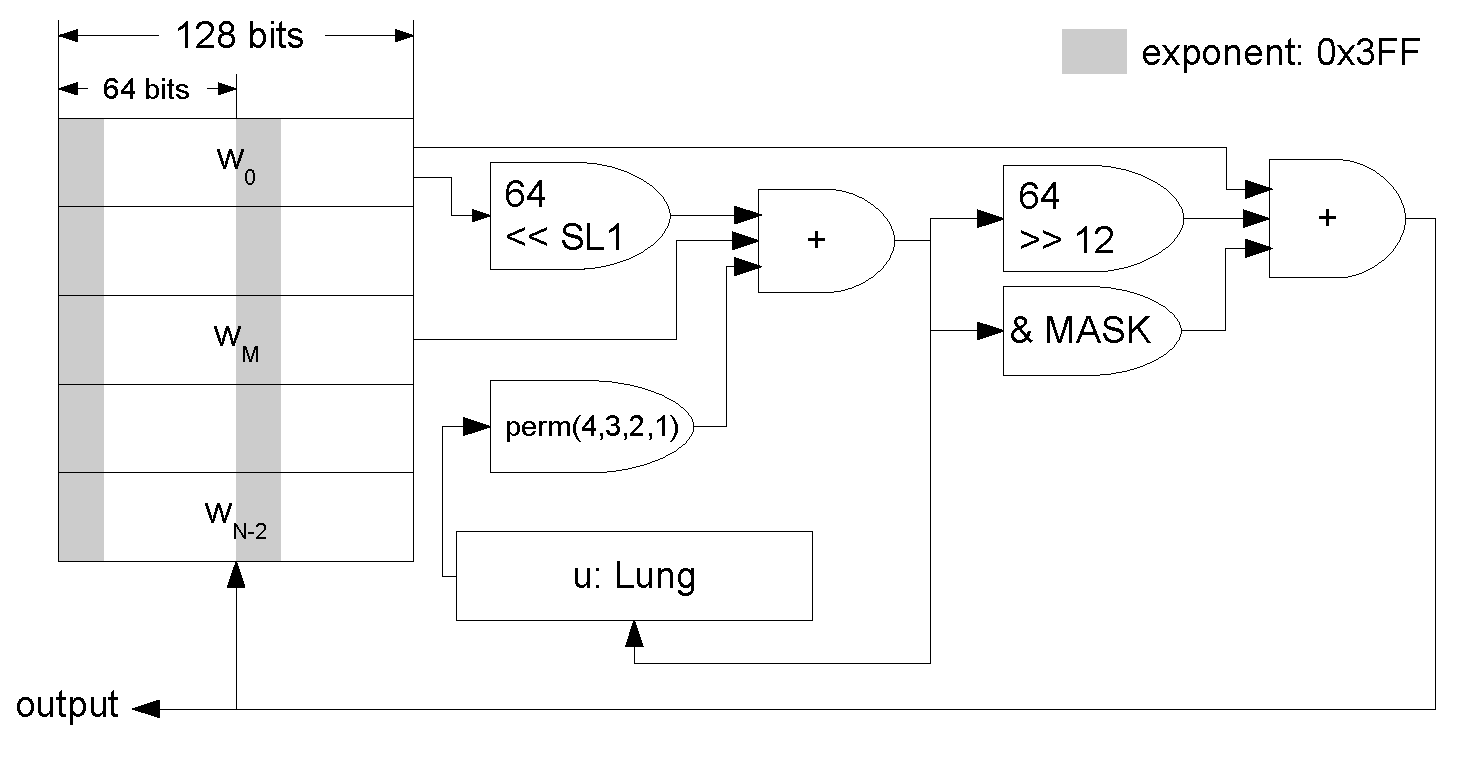
\includegraphics[width=\linewidth]{Saito-fig.pdf}
  \caption{Diagram of dSFMT}
  \label{fig:dsfmt}
\end{figure}

Fig.~\ref{fig:dsfmt} shows the recursion in a circuit-like diagram.
Note that the recursion (\ref{eq:dsfmt}) and (\ref{eq:dsfmt-lung})
is linear, and constant \texttt{0x3ff} (in hexadecimal) of IEEE 754 exponent part
does not appear.
The recursion is carefully selected so that once
the initial values $w_0,\ldots , w_{N-2}$ have \texttt{0x3ff} in their 12 MSBs,
then these constant parts are preserved through the recursion. 
This trick contributes to the generation speed, by avoiding
constant-setting.

Table~\ref{tab:params} lists the parameters 
for dSFMT with various sizes.
Table~\ref{tab:pcv} lists the corresponding fixed points and period
certification vectors(PCV) as discussed in \S\ref{sec:PCV}.

\begin{table}
  \begin{center}
    \caption{Parameter sets. MEXP denotes the Mersenne exponents.
      The column MASK(HIGH) shows the higher
      64-bit of the constant mask, and the column MASK(LOW) shows
      the lower 64-bit in hexadecimal.}
    \label{tab:params}
    \begin{tabular}{rrrrrr} \hline
      MEXP & $N$ & $M$ & SL1 & MASK(LOW) & MASK(HIGH) \\ \hline \hline
      521 & 5 & 3 & 25 & \texttt{0x000fbfefff77efff} 
      & \texttt{0x000ffeebfbdfbfdf} \\
      1279 & 13 & 9 & 19 & \texttt{0x000efff7ffddffee} 
      & \texttt{0x000fbffffff77fff} \\
      2203 & 21 & 7 & 19 & \texttt{0x000fdffff5edbfff} 
      & \texttt{0x000f77fffffffbfe} \\
      4253 & 41 & 19 & 19 & \texttt{0x0007b7fffef5feff} 
      & \texttt{0x000ffdffeffefbfc} \\
      11213 & 108 & 37 & 19 & \texttt{0x000ffffffdf7fffd} 
      & \texttt{0x000dfffffff6bfff} \\
      19937 & 192 & 117 & 19 & \texttt{0x000ffafffffffb3f} 
      & \texttt{0x000ffdfffc90fffd} \\ \hline
    \end{tabular}
  \end{center}
\end{table}

\begin{table}
  \begin{center}
    \caption{Fixed points and period certification vectors (PCVs). 
      Two 64-bit integers (in hexadecimal) piled in one place represent one 128-bit 
      integer with higher (respectively lower) 64-bit being the upper 
      (respectively lower) piled integer. For example, the PCV in the first
      row is \texttt{0xccaa5880000000000000000000000001}.
    }
    \label{tab:pcv}
    \begin{tabular}{c||c|c} \hline
      MEXP & Fixed Point % \multicolumn{1}{c}{Fixed Point} 
      & PCV \\ \hline \hline % \multicolumn{1}{c}{PCV} 
      & \texttt{0xcfb393d661638469} & \texttt{0xccaa588000000000} \\
      521 & \texttt{0xc166867883ae2adb} &\texttt{0x0000000000000001} \\ \hline
      & \texttt{0xb66627623d1a31be} & \texttt{0x7049f2da382a6aeb} \\
      1279 & \texttt{0x04b6c51147b6109b} & \texttt{0xde4ca84a40000001} \\ \hline
      & \texttt{0xb14e907a39338485} & \texttt{0x8000000000000000} \\
      2203 & \texttt{0xf98f0735c637ef90} & \texttt{0x0000000000000001} \\ \hline
      & \texttt{0x80901b5fd7a11c65} & \texttt{0x1ad277be12000000} \\
      4253 & \texttt{0x5a63ff0e7cb0ba74} & \texttt{0x0000000000000001} \\ \hline
      & \texttt{0xd0ef7b7c75b06793} & \texttt{0x8234c51207c80000} \\
      11213 & \texttt{0x9c50ff4caae0a641} & \texttt{0x0000000000000001}\\ \hline
      & \texttt{0x90014964b32f4329} & \texttt{0x3d84e1ac0dc82880} \\
      19937 & \texttt{0x3b8d12ac548a7c7a} & \texttt{0x0000000000000001} \\ 
      \hline
    \end{tabular}
  \end{center}
\end{table}

%%%%%%%%%%%%%%%%%%%%%%%%%%%%%%%%%%%%%%%%%%%%%%%%%%%%%%%%%%%%%%%%%%%%%
\section{Comparison of speed}\label{sec:comp-speed}
We compared generators MT19937, 64-bit MT19937, SFMT19937, dSFMT-old
19937 and dSFMT 19937, each with implementations using and
without using SIMD instructions. For MT and SFMT, `mask' means the
conversion by bit operation described in \S\ref{sec:floating} from 64
bit integer, % of two 32-bit integers,
and `$\times$ const' means the
conversion by multiplying $2^{-64}$. Note that original MT and SFMT
do not use `mask' conversion.

We measured the speeds for five different CPUs: Pentium M 1.4GHz,
Pentium IV 3GHz, core 2 duo 1.83GHz (32-bit mode, use 1 core), AMD
Athlon 64 3800+ (64-bit mode), and PowerPC G4 1.33GHz.  In returning
the random values, we used two different methods.  One is sequential
generation, where one double floating point random number is returned
per call.  The other is block generation, where an array of random
double floating point numbers is generated per call.  We used
Intel C Compiler for intel CPUs (Pentium M, Pentium IV, core 2 duo)
and GNU C Compiler for others (AMD Athlon, Power PC G4).

We measured the consumed cpu-time in second, for $10^8$ generations of
floating point numbers in the range $[0, 1)$ to compare with other
generators. In case of the block generation, we
generate $10^5$ floating point numbers per call, and this is
iterated for $10^3$ times.  For sequential generation, the same $10^8$
floating point numbers are generated, one per call.  We used
the inline declaration {\tt inline} to avoid the function call.
Implementations without SIMD are written in INTERNATIONAL STANDARD
ISO/IEC 9899 : 1999(E) Programming Language-C, Second Edition (which
we shall refer to as C99 in the rest of this article), whereas those
with SIMD use some standard SIMD extension of C99 supported by the
Intel C compiler and GNU C Compiler.

Table~\ref{tab:speed-simd} summarises the speed comparison using SIMD
and Table~\ref{tab:speed-c} shows the speed comparison without using
SIMD.  The 64-bit MT is not listed in Table~\ref{tab:speed-simd}, because
we do not have SIMD version.  The first two lines list the CPU time (in
seconds) needed to generate $10^8$ floating point numbers, for a
Pentium-M CPU.  The first line lists the timings for the
block-generation scheme, and the second line lists those for the
sequential generation scheme. 
The result is that dSFMT is the fastest for all CPUs, all
returning methods, using SIMD and without using SIMD.
Table~\ref{tab:speed-other} shows the speed of other
generators. Although
dSFMT has 52-bit precision while the others have only 32-bit
precision, dSFMT's sequential generation using standard
C (i.e. the slowest case) is faster than the other generators, except xorshift128
\cite{XORSHIFT-MAR}, whose quality is reported to be questionable 
in \cite{XORSHIFT-LEcuyer}.

\begin{table}
  \begin{center}
    \caption{The CPU time (sec.) for $10^8$ generations using SIMD.}
    %of double precision
    %floating point numbers [0, 1) using SIMD feature.}
    \label{tab:speed-simd}
    \begin{tabular}{|ll|r|r|r|r|r|} \hline
      && dSFMT & dSFMT-old & MT & SFMT & SFMT \\
      && (new) & (old) & mask & mask & $\times$ const \\ \hline \hline
      Pentium M & blk & 0.626 & 0.867 & 1.526 & 0.928 & 2.636 \\
      1.4 Ghz & seq & 1.422 & 1.761 & 3.181 & 2.342 & 3.671 \\ \hline
      Pentium 4 & blk & 0.254 & 0.640 & 0.987 & 0.615 & 3.537 \\
      3 Ghz & seq & 0.692 & 1.148 & 3.339 & 3.040 & 3.746 \\ \hline
      core 2 duo & blk & 0.199 & 0.381 & 0.705 & 0.336 & 0.532 \\
      1.83GHz & seq & 0.380 & 0.457 & 1.817 & 1.317 & 2.161 \\\hline
      Athlon 64 & blk & 0.362 & 0.637 & 1.117 & 0.623 & 1.278 \\
      2.4GHz & seq & 0.680 & 0.816 & 1.637 & 0.763 & 1.623 \\ \hline
      PowerPC G4& blk & 0.887 & 1.151 & 2.175 & 1.657 & 8.897 \\
      1.33GHz & seq & 1.212 & 1.401 & 5.624 & 2.994 & 7.712 \\ \hline
    \end{tabular}
  \end{center}
\end{table}

\begin{table}
  \begin{center}
    \caption{The CPU time (sec.) for $10^8$ generations (without using SIMD).}
    %of double precision
    %floating point numbers [0, 1) using standard C (without using SIMD).}
    \label{tab:speed-c}
    \begin{tabular}{|ll|r|r|r|r|r|r|} \hline
      &  & dSFMT & dSFMTold & MT 64 & MT & SFMT & SFMT \\
      &  &(new)&(old)& mask & mask & mask & $\times$ const \\ \hline\hline
      Pentium M & blk & 1.345 & 2.023 & 2.031 & 3.002 & 2.026 & 3.355 \\
      1.4 Ghz & seq & 2.004 & 2.386 & 2.579 & 3.308 & 2.835 & 3.910 \\ \hline
      Pentium 4 & blk & 1.079 & 1.128 & 1.432 & 2.515 & 1.929 & 3.762 \\
      3 Ghz & seq & 1.431 & 1.673 & 3.137 & 3.534 & 3.485 & 4.331 \\ \hline
      core 2 duo & blk & 0.899 & 1.382 & 1.359 & 2.404 & 1.883 & 1.418 \\
      1.83GHz & seq & 0.777 & 1.368 & 1.794 & 1.997 & 1.925 & 2.716 \\ \hline
      Athlon 64 & blk & 0.334 & 0.765 & 0.820 & 1.896 & 1.157 & 1.677 \\
      2.4GHz & seq & 0.567 & 0.970 & 1.046 & 2.134 & 1.129 & 2.023 \\ \hline
      PowerPC G4 & blk & 1.834 & 3.567 & 2.297 & 4.326 & 4.521 & 12.685 \\
      1.33GHz & seq & 1.960 & 2.865 & 4.090 & 5.489 & 5.464 & 9.110 \\ \hline
    \end{tabular}
  \end{center}
\end{table}

\begin{table}
  \begin{center}
    \caption{The CPU time (sec.) for $10^8$ generations for other generators,
       where conversion to floating point numbers uses constant multiplication.}
    % of double precision floating point numbers [0, 1).
    % from 32 bit pseudorandom integers using standard C.}
    \label{tab:speed-other}
    \begin{tabular}{|l|r|r|r|r|} \hline
      & WELL1024 & WELL19937 & MT19937 & XORSHIFT128 \\ \hline
      Pentium M & 2.076 & 2.876 & 2.028 & 1.233 \\
      Pentium 4 & 1.626 & 2.031 & 1.232 & 1.023 \\
      core 2 duo & 1.165 & 1.913 & 1.032 & 0.653 \\
      Athlon 64 & 0.804 & 1.191 & 0.971 & 0.975 \\
      Power PC G4 & 2.947 & 7.524 & 3.082 & 2.267 \\ \hline
    \end{tabular}
  \end{center}
\end{table}

%%%%%%%%%%%%%%%%%%%%%%%%%%%%%%%%%%%%%%%%%%%%%%%%%%%%%%%%%%%%%%%%%%%%%
\section{Dimension of equidistribution}
\label{sec:equidistribution}
We calculated $d(v)$s for our generators, by using method described 
in \S\ref{sec:DE}.
Table~\ref{tab:dd} lists the dimension defects $d(v)$ of dSFMT, for
Mersenne exponent (mexp) $= 521, 1279, 2203, 4253, 11213, 19937$ and
$v=1,2,\ldots, 52$.  The $d(v)$ for $1 \le v \le 22$ are very small. 
The larger mexp
seems to lead to the larger $d(v)$ for $v>22$. Still, the case mexp=19937 has 
total dimension defect $\Delta=2608$, which is smaller than $4188$ of
SFMT19937's 32-bit $\Delta$ and $6750$ of MT19937's 32-bit $\Delta$.
Note that it is natural to guess that 
$\Delta$ increases at least proportionally to the word size $b$,
by its definition (\ref{eq:total-dim-difect}).

\begin{table}
  \begin{center}
    \caption{$d(v)$ $(1 \leq v \leq 52)$ of 52-bit fraction part of dSFMT.}
    \label{tab:dd}
    \begin{tabular}{|r|rrrrrr||r|rrrrrr|} \hline
      & 521 & 1279 & 2203 & 4253 & 11213 & 19937 
      & & 521 & 1279 & 2203 & 4253 & 11213 & 19937 \\ \hline
      d(1) & 0 & 1 & 0 & 0 & 4 & 0 & d(27) & 0 & 0 & 1 & 1 & 33 & 4 \\
      d(2) & 0 & 1 & 1 & 0 & 0 & 1 & d(28) & 0 & 6 & 7 & 28 & 33 & 10 \\
      d(3) & 0 & 2 & 1 & 0 & 0 & 1 & d(29) & 1 & 5 & 7 & 23 & 28 & 67 \\
      d(4) & 0 & 0 & 0 & 0 & 1 & 1 & d(30) & 3 & 3 & 15 & 18 & 80 & 126 \\
      d(5) & 0 & 0 & 0 & 0 & 0 & 0 & d(31) & 2 & 6 & 13 & 15 & 68 & 107 \\
      d(6) & 0 & 1 & 1 & 0 & 1 & 0 & d(32) & 4 & 4 & 10 & 10 & 58 & 88 \\
      d(7) & 0 & 0 & 0 & 0 & 0 & 1 & d(33) & 6 & 12 & 25 & 43 & 120 & 220 \\
      d(8) & 0 & 0 & 0 & 0 & 0 & 1 & d(34) & 6 & 12 & 23 & 44 & 114 & 202 \\
      d(9) & 0 & 1 & 0 & 0 & 0 & 0 & d(35) & 5 & 11 & 21 & 40 & 105 & 185 \\
      d(10) & 1 & 0 & 0 & 0 & 0 & 0 & d(36) & 5 & 10 & 20 & 37 & 96 & 169 \\
      d(11) & 0 & 0 & 0 & 0 & 0 & 0 & d(37) & 5 & 9 & 18 & 33 & 88 & 155 \\
      d(12) & 0 & 0 & 0 & 0 & 0 & 0 & d(38) & 4 & 8 & 16 & 30 & 80 & 141 \\
      d(13) & 0 & 0 & 0 & 0 & 0 & 0 & d(39) & 4 & 7 & 15 & 28 & 72 & 128 \\
      d(14) & 0 & 0 & 0 & 0 & 0 & 1 & d(40) & 4 & 6 & 14 & 25 & 65 & 115 \\
      d(15) & 0 & 0 & 0 & 0 & 0 & 1 & d(41) & 3 & 6 & 12 & 22 & 58 & 103 \\
      d(16) & 0 & 0 & 0 & 0 & 0 & 1 & d(42) & 3 & 5 & 11 & 20 & 51 & 91 \\
      d(17) & 0 & 0 & 0 & 0 & 0 & 0 & d(43) & 3 & 4 & 10 & 17 & 45 & 80 \\
      d(18) & 0 & 0 & 0 & 0 & 0 & 0 & d(44) & 2 & 4 & 9 & 15 & 39 & 70 \\
      d(19) & 0 & 0 & 0 & 0 & 0 & 0 & d(45) & 2 & 3 & 7 & 13 & 34 & 60 \\
      d(20) & 1 & 0 & 0 & 0 & 0 & 0 & d(46) & 2 & 2 & 6 & 11 & 28 & 50 \\
      d(21) & 0 & 0 & 0 & 0 & 7 & 0 & d(47) & 2 & 2 & 5 & 9 & 23 & 41 \\
      d(22) & 0 & 0 & 0 & 0 & 0 & 134 & d(48) & 1 & 1 & 4 & 7 & 18 & 32 \\
      d(23) & 0 & 0 & 7 & 16 & 22 & 94 & d(49) & 1 & 1 & 3 & 5 & 13 & 23 \\
      d(24) & 0 & 1 & 3 & 9 & 19 & 58 & d(50) & 1 & 0 & 3 & 4 & 9 & 15 \\
      d(25) & 0 & 1 & 0 & 6 & 7 & 25 & d(51) & 1 & 0 & 2 & 2 & 4 & 7 \\
      d(26) & 0 & 0 & 0 & 0 & 0 & 0 & d(52) & 1 & 0 & 1 & 0 & 0 & 0 \\ \hline
      \multicolumn{8}{|l|}{total dimension defect $\Delta$} 
      & 73 & 135 & 291 & 531 & 1423 & 2608 \\ \hline
    \end{tabular}
  \end{center}
\end{table}

\begin{remark}
  The number of non-zero terms in $\chi_f(t)$ is an index measuring
  the amount of bit-mixing.  The column ``weight'' in 
  Table~\ref{tab:weight} shows these numbers: 
  dSFMT19937 has the ratio $9756/19992=0.488$ which is higher than those of MT
  (135/19937=0.00677), WELL19937a ($8585/19937=0.431$) and
  WELL19937b ($9679/19937=0.485$).
\end{remark}

\begin{table}[ht]
  \begin{center}
    \caption{The number of non-zero terms in $\chi_f(t)$}
    \label{tab:weight}
    \begin{tabular}{c|rrrrrr} \hline
      mexp & 521 & 1279 & 2203 & 4253 & 11213 & 19937 \\
      degree of $\chi_f(t)$ & 544 & 1376 & 2208 & 4288 & 11256 & 19992 \\
      weight & 273 & 673 & 1076 & 2233 & 5684 & 9756 \\ 
      ratio & 0.50 & 0.49 & 0.49 & 0.52 & 0.50 & 0.49 \\ \hline
    \end{tabular}
  \end{center}
\end{table}
%%%%%%%%%%%%%%%%%%%%%%%%%%%%%%%%%%%%%%%%%%%%%%%%%%%%%%% 
% %\subsection{Trade-off between speed and quality}
% It is difficult to measure the generation speed of a PRNG in a fair way,
% since it depends heavily on the circumstances. 
% The 
% WELL \cite{WELL} generators have the best possible dimensions of 
% equidistribution (i.e. $\Delta=0$)
% for various periods ($2^{1024}-1$ to $2^{19937}-1$).
% %If we use the function call to PRNG
% If we use the function call to the PRNG
% for each generation, then a large part of the CPU time
% is consumed for handling the function call, and in the 
% experiments in \cite{WELL} or \cite{XORSHIFT}, WELL 
% is not much slower than MT. On the other hand, if we avoid
% the function call, WELL is slower than MT for some CPUs, 
% as seen in Table~\ref{tab:speed}. 

% Since $\Delta=0$, WELL has a better quality than MT or SFMT
% in a theoretical sense. 
% However, one may argue whether this difference is 
% observable or not. In the case of an $\bbf2$-linear generator,
% the dimension of equidistribution $k(v)$ of $v$-bit accuracy
% means that
% there is no constant linear relation among the 
% $kv$ bits, but there exists a linear relation among
% the $(k+1)v$ bits, where $kv$ bits 
% ($(k+1)v$ bits) are taken from
% all the consecutive $k$ integers 
% ($k+1$ integers, respectively)
% by extracting the $v$ MSBs from each.
% However, the existence of a linear relation does not necessarily
% mean the existence of some observable bias.
% According to \cite{TESTWEIGHT}, it requires $10^{28}$
% samples to detect an $\bbf2$-linear relation with 
% 15 (or more) terms among 521 bits, by weight distribution test. 
% If the number of 
% bits is increased, 
% the necessary sample size is increased rapidly. Thus, it seems
% that $k(v)$ of SFMT19937 is sufficiently large, far beyond
% the level of the observable bias. 
% On the other hand, the speed of the generator is 
% observable.
% Thus, SFMT focuses more on the speed, for applications
% that require fast generations. 
% (Note: the referee pointed out that statistical
% tests based on the rank of $\bbf2$-matrix is sensitive to 
% the linear relations \cite{TESTU01}, 
% so the above observation is not necessarily true.)

% %\subsection{Trade-off between speed and portability}\label{sec:portability}
% There is a trade-off between the speed and portability.
% %We prepare (1) a standard C code of SFMT, which uses 
% We prepared (1) a standard C code of SFMT, which uses 
% functions specified in C99 only, (2) an optimized C code for
% Intel Pentium SSE2, and 
% (3) an optimized C code for PowerPC AltiVec. The optimized codes require
% %icl (Intel C Compiler) or gcc compiler with suitable options.
% the icl (Intel C Compiler) or gcc compiler with suitable options.

The dSFMT generators passed the DIEHARD statistical tests \cite{diehard}.
They also passed TestU01 \cite{TESTU01} consisting of
144 different tests, except for 
\texttt{LinearComp} (fail unconditionally) and 
MatrixRANK tests (fail if the size of dSFMT is smaller then 
the matrix size). These tests measure ${\mathbb F}_2$-linear 
dependency of the outputs, and reject ${\mathbb F}_2$-linear generators, 
such as MT, SFMT and WELL.
%(We comment that for the tests on random integers, 
%the least 32-bits are tested.)

We shall keep the latest version of the codes in the web page \cite{web:SFMT}.


\begin{acknowledgement}
This study is partially
supported by JSPS/MEXT Grant-in-Aid for Scientific Research
No.19204002, No.18654021, and JSPS Core-to-Core Program
No.18005. The second author is partially supported
as a visiting professor of The Institute of Statistical 
Mathematics. The authors are thankful to the anonymous 
referees and the editor for valuable comments.
\end{acknowledgement}

\bibliographystyle{plain}
%\bibliography{sfmt-kanren}
\begin{thebibliography}{10}

\bibitem{BRENT}
R.P. Brent and P.~Zimmermann.
\newblock Random number generators with period divisible by a {Mersenne} prime.
\newblock In {\em Computational Science and its Applications - ICCSA 2003},
  volume 2667, pages 1--10, 2003.

\bibitem{BRENT-PRIM}
R.P. Brent and P.~Zimmermann.
\newblock Algorithms for finding almost irreducible and almost primitive
  trinomials.
\newblock {\em Fields Inst. Commun.}, 41:91--102, 2004.

\bibitem{CLT}
R.~Couture, P.~L'Ecuyer, and S.~Tezuka.
\newblock On the distribution of k-dimensional vectors for simple and combined
  {Tausworthe} sequences.
\newblock {\em Math. Comp.}, 60(202):749--761, 1993.

\bibitem{web:Fog}
Agner Fog.
\newblock Pseudo random number generators.
\newblock \url{http://www.agner.org/random/}.

\bibitem{FUSHIMI90}
M.~Fushimi.
\newblock Random number generation with the recursion $x_t = x_{t-3p}\oplus
  x_{t-3q}$.
\newblock {\em Journal of Computational and Applied Mathematics}, 31:105--118,
  1990.

\bibitem{ieee754}
{IEEE} standard for binary floating-point arithmetic 754, 2008.
\newblock \url{http://ieeexplore.ieee.org/servlet/opac?punumber=4610933}.

\bibitem{knuth:bible}
D.~E. Knuth.
\newblock {\em The Art of Computer Programming. Vol.2. Seminumerical
  Algorithms}.
\newblock Addison-Wesley, Reading, Mass., 3rd edition, 1997.

\bibitem{COMBTAUS}
P.~L'Ecuyer.
\newblock Maximally equidistributed combined tausworthe generators.
\newblock {\em Math. Comp.}, 65(213):203--213, 1996.

\bibitem{LEcuyer-combdif}
P.~L'Ecuyer and J.~Granger-Pich\'{e}.
\newblock Combined generators with components from different families.
\newblock {\em Mathematics and Computers in Simulation}, 62:395--404, 2003.

\bibitem{F2RNG-LEcuyer}
P.~L'Ecuyer and F.~Panneton.
\newblock $\mathbb{F}_2$-linear random number generators.
\newblock In {\em Advancing the Frontiers of Simulation: A Festschrift in Honor
  of George Samuel Fishman}, pages 175--200, 2009.
\newblock C. Alexopoulos, D. Goldsman, and J. R. Wilson Eds.

\bibitem{TESTU01}
P.~L'Ecuyer and R.~Simard.
\newblock {TestU01}: {A} {C} library for empirical testing of random number
  generators.
\newblock {\em ACM Transactions on Mathematical Software}, 15(4):346--361,
  2006.

\bibitem{diehard}
G.~Marsaglia.
\newblock {The Marsaglia Random Number CDROM, with the DIEHARD Battery of Tests
  of Randomness.}
\newblock Department of Statistics, Florida State University, (1996)
  \url{http://www.stat.fsu.edu/pub/diehard/}.

\bibitem{XORSHIFT-MAR}
G.~Marsaglia.
\newblock Xorshift {RNGs}.
\newblock {\em Journal of Statistical Software}, 8(14):1--6, 2003.

\bibitem{MT}
M.~Matsumoto and T.~Nishimura.
\newblock Mersenne twister: A 623-dimensionally equidistributed uniform
  pseudorandom number generator.
\newblock {\em ACM Trans. on Modeling and Computer Simulation}, 8(1):3--30,
  January 1998.
\newblock \url{http://www.math.sci.hiroshima-u.ac.jp/~m-mat/MT/emt.html}.

\bibitem{MT64}
T.~Nishimura.
\newblock Tables of 64-bit mersenne twisters.
\newblock {\em ACM Trans. on Modeling and Computer Simulation}, 10(4):348--357,
  October 2000.

\bibitem{XORSHIFT-LEcuyer}
F.~Panneton and P.~L'Ecuyer.
\newblock On the {Xorshift} random number generators.
\newblock {\em ACM Transactions on Modeling and Computer Simulation},
  15(4):346--361, 2005.

\bibitem{WELL}
F.~Panneton, P.~L'Ecuyer, and M.~Matsumoto.
\newblock Improved long-period generators based on linear reccurences modulo 2.
\newblock {\em ACM Transactions on Mathematical Software}, 32(1):1--16, 2006.

\bibitem{web:SFMT}
M.~Saito and M.~Matsumoto.
\newblock {SFMT Homepage}.
\newblock
  \url{http://www.math.sci.hiroshima-u.ac.jp/~m-mat/MT/SFMT/index.html}.

\bibitem{SFMT}
M.~Saito and M.~Matsumoto.
\newblock {SIMD}-oriented fast {Mersenne} twister : a 128-bit pseudorandom
  number generator.
\newblock In {\em Monte Carlo and Quasi-Monte Carlo Methods 2006}, LNCS, pages
  607--622. Springer, 2008.

\bibitem{wiki:SIMD}
{SIMD From Wikipedia, the free encyclopedia}.
\newblock \url{http://en.wikipedia.org/wiki/SIMD}.

\end{thebibliography}
\end{document}
%%%%%%%%%%%%%%%%%%%%%%%%%%%%%%%%%%%%%%%%%%%%%%%%%%%%%%%%%%%%%%%%%%%%%
% LocalWords:  MCQMC denormalized xxxx NaN xxxxx Hiroshi Haramoto MCM nw RTM tI
% LocalWords:  wN th wr wo PCV kv vk sl rrrrrrr MEXP fbfefff efff ffeebfbdfbfdf
% LocalWords:  ffddffee fbffffff fff fdffff edbfff fffffffbfe fffef feff fffd
% LocalWords:  ffdffeffefbfc ffffffdf dfffffff bfff ffafffffffb ffdfffc rr xcfb
% LocalWords:  xccaa xc ae adb xb da aeb xde xf ef fd cb ba xd caae uint IEC le
% LocalWords:  icl dSFMTv const blk Ghz mexp rrrrrr sfmt kanren equi LSB intel
% LocalWords:  crrrrrr ap ar xorshift Im dSFMT's Agner precomputing PCVs cpu
% LocalWords:  dSFMTold DIEHARD TestU LinearComp MatrixRANK
